\section{Superposition}
\label{sec:super}

\subsection{The fringe law}
\label{sec:fringe}

The rest of the paper rests on one observation about where the visible pattern
of a superposition comes from.

Fix a point $p$ and let $D=\idx_1-\idx_2$ be the difference of index fields. Write
$w_i$ for layer $i$'s stroke half-width measured \emph{in index units},
$w_i=h_i\lVert\nabla\idx_i\rVert$, and $b_i=a\lVert\nabla\idx_i\rVert$ for its
band. Define the index-space stroke profile
$A_i(u)=1-\mathrm{smoothstep}(w_i-b_i,\,w_i+b_i,\,\mathrm{pd}(u,1))$.

\begin{theorem}[Fringe law]
\label{thm:fringe}
Let $u$ be the direction of the mean index gradient
$g=\tfrac12(\nabla\idx_1+\nabla\idx_2)$, let $T=1/\lVert g\rVert$ be the carrier
period, and let $S=p+[-T/2,T/2]\,u$. Suppose that on $S$ both families are local
foliations, that both gradients $\nabla\idx_i$ are constant, and that $D$ is
constant. Then the mean ink over $S$ is
\begin{equation}
  \label{eq:phi}
  \begin{gathered}
    \bar\alpha(p) \;=\; \Phi\big(D(p)\big), \qquad\text{where}\\
    \Phi(\Delta) \;=\; \int_0^1 \Big[A_1(v)+A_2(v-\Delta)-A_1(v)A_2(v-\Delta)\Big]\,\mathrm{d}v,
  \end{gathered}
\end{equation}
which depends on $p$ only through $D(p)$. If $D$ is not constant on $S$, the
same expression holds up to an error $O(\het)$ in the ratio \eqref{eq:ratio}
below; if the gradients are merely near-constant, the error grows with their
variation across $S$. In the hard-edged limit $b_i\to0$, provided
$w_1+w_2\le\tfrac12$,
\begin{equation}
  \begin{split}
    \Phi(\Delta) = {}&2w_1+2w_2 \\
      &{}-\min\!\big(2\min(w_1,w_2),\,\max(0,\,w_1+w_2-\mathrm{pd}(\Delta,1))\big):
  \end{split}
  \label{eq:tent}
\end{equation}
a saturating tent in $D$: flat at $2\max(w_1,w_2)$ while one stroke lies
inside the other ($\mathrm{pd}(D,1)\le|w_1-w_2|$), rising with unit slope, and
saturating at $2w_1+2w_2$ once the strokes clear each other. For equal widths
the floor is a single point and the profile is the familiar tent. (Past
$w_1+w_2=\tfrac12$ the strokes also overlap across the far side of the period
and a second overlap term appears; the integral form \eqref{eq:phi} carries it
automatically.)
\end{theorem}

The proof is a change of variables and is given in Appendix~\ref{app:fringe}; the
content is entirely in the statement. The hypotheses are not interchangeable,
and it pays to be exact about them. ``Both families are local foliations on
$S$'' is what lets us reparameterize the segment by index instead of by
arclength. Constant gradients are what make the stroke widths $w_i$ constants
and the reparameterization measure-preserving; drop that hypothesis and the
conclusion fails even with $D$ exactly constant, which is why the verification
below excludes samples whose gradient varies across a period. ``$D$ is constant
on $S$'' is what makes the answer a function of $D(p)$ alone, and it is the
strong one: exact constancy means the two carriers agree exactly in pitch and
direction, so the interesting cases only satisfy it approximately. The appendix
carries the general case through and shows the correction is first order in
$\het$, which is the same small parameter \S\ref{sec:visibility} uses to decide
whether a fringe exists at all. So the theorem is exact in the limit that a
fringe becomes infinitely broad, and degrades in the parameter that measures how
far from that limit we are, which is why the verification below both
restricts to $\het\le1/4$ and reports the residual rather than claiming zero.
Four further remarks.

\paragraph{The locus and the profile shape are classical; the statement is not.}
$\Phi$ is periodic with period $1$ and extremal at $D\in\Z$ and
$D\in\Z+\tfrac12$. So the light fringes are exactly $\{D\in\Z\}$ (where the two
families' members locally coincide and their strokes overlap, wasting ink) and
the dark fringes are exactly $\{D\in\Z+\tfrac12\}$, where the members interleave
and the ink is maximally spread. The moir\'e is the contour plot of
$\idx_1-\idx_2$ at unit interval, and nothing else about either family survives
the average.

Both halves of that sentence have classical ancestors, and we want to be exact
about the debt. The locus: writing the two families as $\idx_1=m$, $\idx_2=n$
and asking where members cross in a fixed relation $m-n=k$ is the \emph{indicial
equation} of Oster, Wasserman and Zwerling~\cite{Oster1964}, which Amidror
presents as the geometric approach~\cite{Amidror2009Theory}; read backwards it
is the fringe-order law of moir\'e interferometry~\cite{Post2008Moire}. The
profile: for two black layers Eq.~\ref{eq:alpha} composes as a union, so the
transmittances multiply, and \eqref{eq:phi} can be rewritten as
\begin{equation}
  \Phi(\Delta) \;=\; 1-\big(T_1\star T_2\big)(\Delta),
  \qquad T_i = 1-A_i,
  \label{eq:tconv}
\end{equation}
the circular cross-correlation of the two transmittance profiles, which for
periodic gratings is Amidror's T-convolution
theorem~\cite{Amidror1994TConv, Amidror2009Theory}, and which for binary
gratings yields exactly the trapezoid of \eqref{eq:tent}, a shape known since
Patorski et al.~\cite{Patorski1976Profile}; Harthong reached the same profile by
local averaging~\cite{Harthong1981Moire}, and Amidror and Hersch extended it to
curved layers as the profile composed with the index
difference~\cite{Amidror1998Fourier}. Metrology, likewise, has read intensity
between fringes as fractional fringe order since
Sciammarella~\cite{Sciammarella1965Basic}.

What Theorem~\ref{thm:fringe} contributes is the statement itself. The
classical results are Fourier identities about fixed global profiles composed
with closed-form bending functions, with the visible moir\'e identified
perceptually; the theorem is an exact local spatial mean of the actual
compositing operator, with stated hypotheses and a first-order error bound in a
computable parameter. Its stroke widths $w_i=h_i\lVert\nabla\idx_i\rVert$ vary
across the frame, so the profile is a per-pixel family rather than one function.
It applies to an index field that exists only as the output of a search
(\S\ref{sec:walking}), where no bending function can be written down. And it
comes with $\het$ (\S\ref{sec:visibility}), a validity criterion tied to the
theorem's own error term rather than to a visibility argument, which varies over
the frame and can be drawn. Because $\Phi$ is a formula for averaged ink rather
than a set of curves, it can also be \emph{drawn} (\S\ref{sec:envelope}) and
\emph{inverted} (\S\ref{sec:beyond}); those are the parts we lean on.

\paragraph{The tent saturates, and the saturation is a design fact.}
Eq.~\ref{eq:tent} is piecewise linear with a flat top, reached as soon as
$\mathrm{pd}(D,1)>w_1+w_2$: most of the fringe is at full contrast, and the
transition occupies only a $(w_1{+}w_2)$-wide sliver of each period, which is
why field-composited moir\'e looks crisper than a first-harmonic model
predicts. It also explains a design behavior we had noticed but not
understood: past a certain stroke thickness, thickening the strokes stops changing the
fringe and only darkens the whole frame. The dependence on stroke widths is the
classical opening-ratio dependence of the trapezoid, here live under a slider.

\paragraph{No periodicity is required, and no closed form either.}
$\idx_1$ and $\idx_2$ are arbitrary. The theorem's hypotheses are local
(affineness of $D$ over one carrier period, and the eikonal condition) and say
nothing about global structure. A spiral is admissible. Two hyperbola families are
admissible. So, more delicately, is a \emph{walking} family
(\S\ref{sec:walking}), whose index field exists without having a formula.
Wherever consecutive members bracket the point (everywhere when the drift
stays below the spacing, and away from the family's envelope curves
otherwise), the nearest index $n^\star$ plus the fractional residual
$h_p(n^\star)/(h_p(n^\star)-h_p(n^\star{+}1))$ is a continuous scalar field whose
level sets are exactly the members. It is an index field computed by search
rather than written down, the theorem does not care about the difference, and
the \texttt{walking-circle} row of Table~\ref{tab:fringe} measures the law
holding on it.

\paragraph{The difference is one character among many.}
Nothing fixes a family's index convention: relabel its members by any affine
integer map and $\idx$ changes while every curve, stroke and pixel stays the
same. $D=\idx_1-\idx_2$ is therefore one representative of a lattice of
candidate beats (the integer combinations $k_1\idx_1+k_2\idx_2$, each a
\emph{character} of the pair), and the theorem holds for whichever character
makes its own hypothesis true: the one that is slow against the carriers.
$k=(1,1)$ is the classical \emph{sum} moir\'e~\cite{Oster1964}: where the two
index gradients anti-align it is the sum that beats slowly, and a
difference-only reading misses fringes that stand in plain sight. (Our first
envelope view held $\idx_1-\idx_2$ fixed while it averaged, and every
sum-labeled fringe system in the frame vanished from it.) Higher orders are
just as classical: two line families near a $2{:}1$ pitch ratio beat in
$2\idx_1-\idx_2$, fainter but plainly
visible~\cite{Amidror1994TConv, Amidror2009Theory}, and the same trap
recurs one level up: a criterion that scans only $k=(1,\mp1)$ declares such a
frame fringe-free while the fringe stands in the render.
\S\ref{sec:visibility} folds the low-order characters into one criterion
(Figure~\ref{fig:hills} draws two of them as height functions over one
superposition), the envelope sweeps orthogonally to whichever one the
criterion picks, and for lattice layers, whose index is a vector, the same
characters range over integer combinations of generators (supplemental \S S3).

\begin{figure*}[t]
  \centering
  \begin{tikzpicture}
    % A ground behind the (transparent) render. It is the page's own white: the
    % floors carry their own warm tint inside the render, so nothing floats
    % without a tinted block here, and this was the only figure in the paper that
    % brought its own background colour to the page. Shrink it by moving these two
    % corners; put a colour back here if the render is ever made fully opaque.
    \fill[white]
      (0,0) rectangle (\linewidth,0.39972\linewidth);
    \node[anchor=south west, inner sep=0] (img) at (0,0)
      {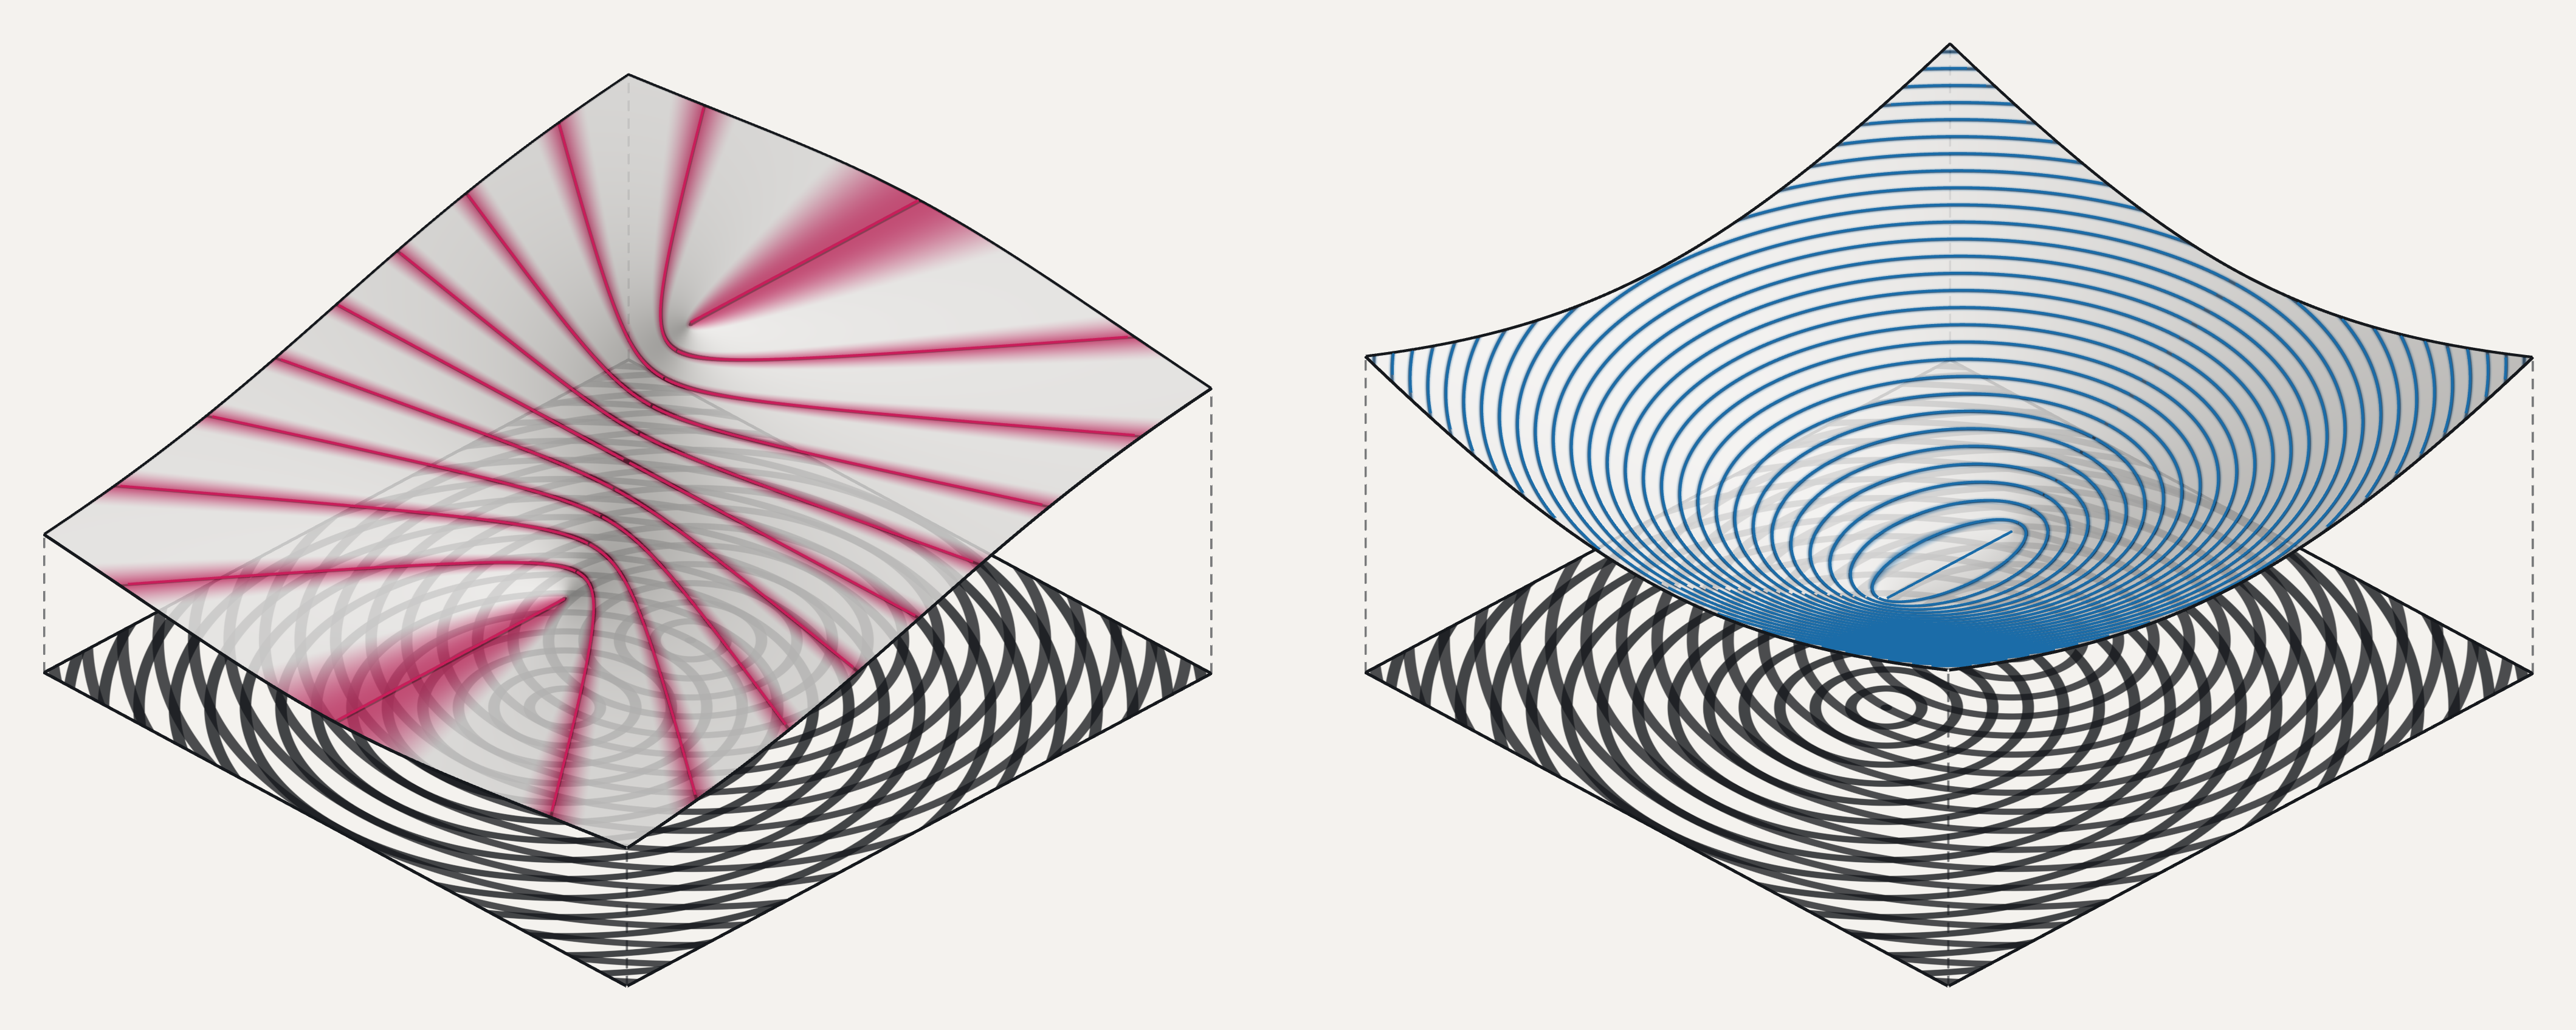
\includegraphics[width=\linewidth]{figures/charhills}};
    \begin{scope}[shift={(img.south west)},
        x={($ (img.south east)-(img.south west) $)},
        y={($ (img.north west)-(img.south west) $)}]
      \tikzset{lab/.style={font=\footnotesize, inner sep=1pt}}
      \tikzset{lead/.style={-{Stealth[length=4.5pt]}, line width=0.55pt}}
      \node[lab, text=ink, align=left, anchor=west] (gl) at (0.0114,0.8285)
        {the graph of\\$D=\idx_1-\idx_2$};
      \draw[lead, ink!65] (gl.south) to[out=-69,in=132] (0.0905,0.607);
      \node[lab, text=accent!88!ink, anchor=west] (cl) at (0.3873,0.8567)
        {contours at $D\in\Z$};
      \draw[lead, accent!75] (cl.south) to[out=-155,in=90] (0.4113,0.6706);
      \node[lab, text=ink!70, anchor=west] (rl) at (0.0586,0.0309)
        {two ring families};
      \draw[lead, ink!55] (rl.east) to[out=10,in=205] (0.278,0.110);
      \node[lab, text=cool!90!ink, anchor=east] (sl) at (0.9769,0.8754)
        {the sum $\idx_1+\idx_2$};
      \draw[lead, cool!75] (sl.south) to[out=-109,in=76] (0.8817,0.7531);
    \end{scope}
  \end{tikzpicture}
  \Description{Two orthographic 3D renders side by side. In each, a floor
  patch carries two superposed families of fine concentric rings whose
  overlap forms a moire, and a translucent surface floats above it, joined
  to the floor by dashed vertical corner posts. Left: the surface is the
  graph of the index difference, a twisted sheet carrying broad crimson
  bands that widen where the sheet lies flat and crowd into a wall between
  the ring centers; labels read the graph of D, contours at integer D,
  and two ring families. Right: the same floor under the graph of the
  index sum, a bowl covered in tightly crowded blue rings with one bold
  flat bar between the centers, labeled the sum.}
  \caption{\figlead{Characters as hills over the pattern.}
  Two identical ring families (floor); above them, the graph of an integer
  character of their indices, its integer levels drawn on the surface.
  \textbf{Left:} the difference $D=\idx_1-\idx_2$. Its levels are the
  confocal hyperbolae; where the sheet lies flat they spread into the broad
  fringes the eye picks out of the moir\'e below, and on the steep wall
  between the centers they crowd at the carrier's own scale. \textbf{Right:}
  the sum $\idx_1+\idx_2$ over the same floor is steep nearly everywhere: its
  levels crowd into texture, no broad fringe forms, and the one flat
  stretch, the inter-focal segment, carries the sum's one visible fringe.
  The criterion of \S\ref{sec:visibility} is this comparison made pointwise:
  the visible moir\'e is the character whose hill lies flattest, weighted by
  the contrast its order costs (\S\ref{sec:selection}).}
  \label{fig:hills}
\end{figure*}

\subsection{When is there a fringe at all?}
\label{sec:visibility}

Theorem~\ref{thm:fringe} needs $D$ to be nearly constant over one carrier
period, and a beat is worth calling a fringe only when it is broad against that
period. Both requirements are the same ratio. Define the \emph{heterodyne ratio}
\begin{equation}
  \het(p) = \frac{\lVert\nabla D(p)\rVert}{\lVert g(p)\rVert}
  = \frac{\lVert\nabla\idx_1-\nabla\idx_2\rVert}
         {\big\lVert\tfrac12(\nabla\idx_1+\nabla\idx_2)\big\rVert}.
  \label{eq:ratio}
\end{equation}
$D$ changes by $\het$ across one carrier period, so $\het\ll1$ is exactly the
condition that a fringe be large compared with the carrier;
Figure~\ref{fig:hills} draws it as the flatness of $D$'s graph against the
carriers' slope. Its numerator is the
classical local moir\'e frequency, the vector difference of the two local
carrier frequencies~\cite{Amidror2009Theory}, made a per-pixel \emph{field},
so it varies over the frame and can be drawn (Figure~\ref{fig:visibility}).
(``Heterodyne'' is borrowed from radio practice; in interferometry the word
names a temporal frequency offset, which this is not.)

Equation \eqref{eq:ratio} is the $k=(1,-1)$ instance of the character family of
\S\ref{sec:fringe}: for a general integer pair $k=(k_1,k_2)$,
\begin{equation}
  \het_k(p) \;=\;
  \frac{\lVert k_1\nabla\idx_1+k_2\nabla\idx_2\rVert}
       {\tfrac12\lVert k_1\nabla\idx_1-k_2\nabla\idx_2\rVert},
  \label{eq:ratiok}
\end{equation}
whose denominator is the mean carrier gradient in the relabeling that brings
the carriers close. The pair $(1,\mp1)$
recovers the difference and sum moir\'es~\cite{Oster1964, Amidror2009Theory};
where the two gradients anti-align the difference ratio diverges while a bold
sum fringe stands in plain sight, and the higher pairs catch the
rational-pitch beats the same way~\cite{Amidror1994TConv}. Slowness alone,
though, cannot rank the candidates: good rational approximations exist at
every order, so the bare minimum of \eqref{eq:ratiok} over all $k$ favors
beats no ink can carry. The beat at $k$ rides layer $1$'s
$\lvert k_1\rvert$th harmonic against layer $2$'s $\lvert k_2\rvert$th, and a
stroke profile's harmonics decay like $1/m$, so its contrast falls like
$1/\lvert k_1k_2\rvert$. The operative criterion is therefore the
\emph{weighted} merit
\begin{equation}
  \mu_k \;=\; \lvert k_1 k_2\rvert\,\het_k,
  \label{eq:merit}
\end{equation}
minimized over the characters; $\mu_{(1,\mp1)}=\het_{(1,\mp1)}$, so the
classical criterion is the order-one slice, and the weight doubles as the
tie-breaker that keeps a near-tie from flickering toward the fainter beat.
Which characters must be scanned is not a perceptual question, and
\S\ref{sec:selection} answers it exactly. \Moire{} draws the minimum live, as
a view toggled beside the envelope, and hands the winning character to the
envelope's sweep, so an author sees where a fringe will form, and which beat
it is, before committing to the parameters.

\begin{figure*}[t]
  \centering
  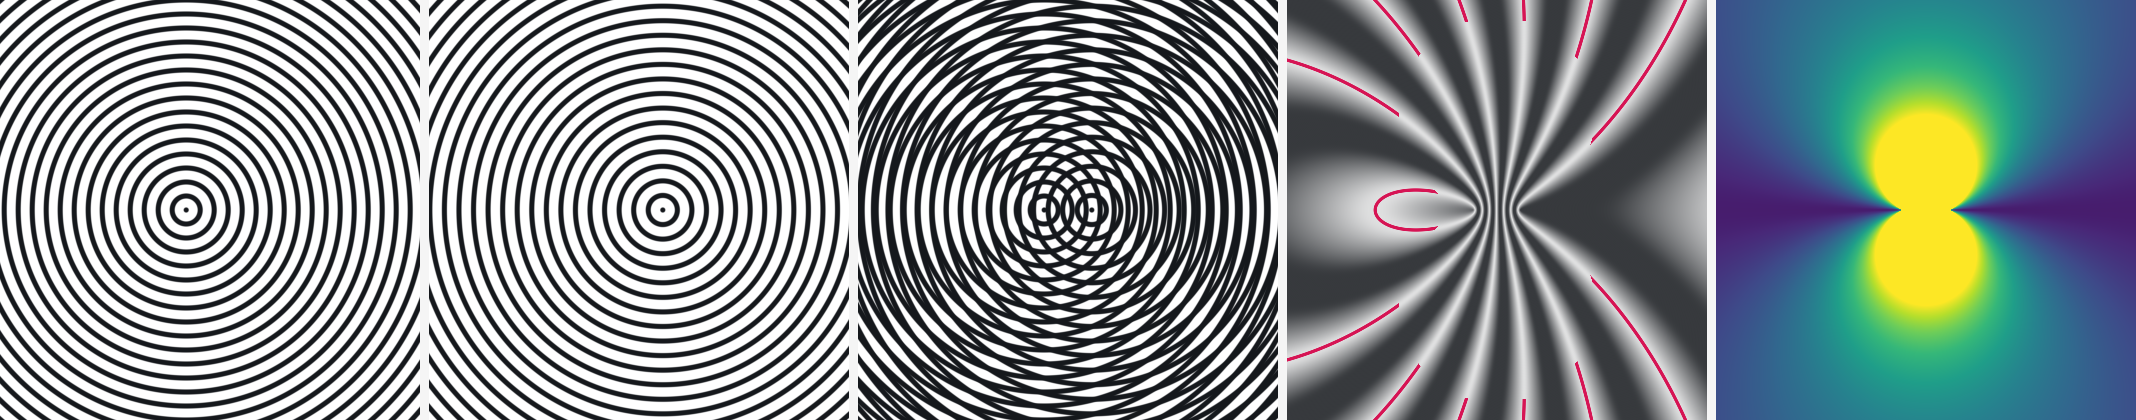
\includegraphics[width=\linewidth]{figures/fringe-law.png}
  \panelrow{0.19663}{0.00421}{%
    (a) layer $1$,
    (b) layer $2$,
    (c) superposition,
    (d) averaged ink\, $+\;\{D\in\Z\}$,
    (e) heterodyne ratio $\het$}
  \Description{Five square panels. The first two are black-on-white concentric rings
  about slightly different centers. The third overlays them and shows large curved
  bands cutting across the rings. The fourth is a smooth gray field of broad light
  and dark bands fanning out from the center, its light bands traced by thin crimson
  curves that stop short of two blank lobes either side of center. The fifth is a
  blue-to-yellow heat map of the same frame, dark blue over most of it with two
  bright yellow lobes where the crimson curves stopped.}
  \caption{\figlead{The moir\'e is a contour plot of the index difference.}
  \textbf{(a,\,b)} Two circle families, rendered alone from their own distance
  fields. Their centers differ by $34$ units and their pitches by four percent, and
  nothing else. \textbf{(c)} Their superposition, in which a fringe system appears
  that is in neither layer. \textbf{(d)} The theorem is a statement about averaged
  ink, so this is that average: the envelope view of \S\ref{sec:envelope}, which
  integrates the same two fields over one period of their common phase and so
  removes the carriers without blurring anything, with the unit level sets of
  $D=\idx_1-\idx_2$ laid over it in crimson. Those curves are computed from the two
  index fields alone and never from the image, and they land on the light fringes.
  They are drawn only where
  $\het\le1/4$, which is why they stop short of the two lobes flanking the centers.
  \textbf{(e)} The heterodyne ratio $\het$ of Eq.~\ref{eq:ratio} over the same
  frame, dark where Theorem~\ref{thm:fringe} applies and bright where the two
  carriers are too different for a fringe to exist. The bright lobes are the
  region the overlay declines to describe, and in the superposition they are
  the region that reads as a rosette of crossings rather than as bands.}
  \label{fig:visibility}
\end{figure*}

We take $\min_k\mu_k\le1/4$ as the operational definition of the fringe
regime.

\subsection{Which beat wins is best approximation}
\label{sec:selection}

Fix a point and ask which character minimizes \eqref{eq:merit} as ever higher
orders are admitted. In one dimension the answer is a classical theorem. Two
parallel families of pitches $s_1$, $s_2$ have collinear index gradients of
magnitudes $1/s_1$, $1/s_2$, so the character $(p,-q)$ beats at spatial
frequency $\lvert p/s_1-q/s_2\rvert=(1/s_1)\,\lvert q\rho-p\rvert$ with
$\rho=s_1/s_2$ the pitch ratio: slowness \emph{is} rational approximation
error. The characters that set a new slowness record as the order budget
grows are the best approximations of $\rho$ of the second kind, and by
Lagrange's theorem those are exactly the convergents of its continued
fraction~\cite{Khinchin1964Continued}. The visible-beat hierarchy of a
two-pitch superposition is the continued fraction of its pitch ratio: the
$2{:}1$ beat is a convergent, the $3{:}1$ beat is the next one, and the
golden ratio, whose convergents converge slowest of all
rationals~\cite{Hurwitz1891Annaherung}, is the fringe desert. We verified the
identification numerically over $\selRatios$ pitch ratios (the named
constants plus a deterministic random spread): every record-setting character
is a convergent, with no exceptions
(\texttt{tools\pslash exp\pslash convergents.mjs}). The envelope's own
quasi-random tap rule (supplemental \S S3) is this theorem run backwards: its
scrambled generator advances by the golden ratio precisely so that \emph{no}
integer character can survive the average.

\begin{figure*}[t]
  \centering
  % The two panels are sized so their printed heights agree: the strip is
  % 1440 x 540, so at 0.61\textwidth it stands 0.229\textwidth tall, and the
  % axis height below is chosen to match it, labels included.
  \begin{subfigure}[b]{0.37\textwidth}
    \begin{tikzpicture}
      \begin{axis}[paperaxis, height=3.62cm, width=\linewidth,
        xlabel={pitch ratio $\rho$}, ylabel={locked ratio $p/q$},
        xmin=1, xmax=3.5, ymin=0.9, ymax=3.6,
        ytick={1,1.5,2,2.5,3},
        yticklabels={$1$,$\tfrac32$,$2$,$\tfrac52$,$3$},
        legend columns=4,
        legend style={at={(0.5,1.03)}, anchor=south, draw=none, fill=none},
      ]
        \addplot[soft!45, thin, forget plot, domain=1:3.5] {x};
        \addplot[soft, densely dashed, thin, forget plot] coordinates
          {(1.6180339,0.9) (1.6180339,3.6)};
        \node[soft, font=\scriptsize, anchor=south west] at (axis cs: 1.628, 3.18)
          {$\varphi$};
        \addplot[ink!30, const plot, line width=1.1pt]
          table [x=rho, y expr=\thisrow{p2}/\thisrow{q2}, col sep=comma]
          {data/convergent-fan.csv};
        \addlegendentry{$q\le2$}
        \addplot[cool, const plot, line width=0.85pt]
          table [x=rho, y expr=\thisrow{p4}/\thisrow{q4}, col sep=comma]
          {data/convergent-fan.csv};
        \addlegendentry{$q\le4$}
        \addplot[warm, const plot, line width=0.6pt]
          table [x=rho, y expr=\thisrow{p8}/\thisrow{q8}, col sep=comma]
          {data/convergent-fan.csv};
        \addlegendentry{$q\le8$}
        \addplot[accent, const plot, line width=0.45pt]
          table [x=rho, y expr=\thisrow{p16}/\thisrow{q16}, col sep=comma]
          {data/convergent-fan.csv};
        \addlegendentry{$q\le16$}
      \end{axis}
    \end{tikzpicture}
    \caption{the convergent staircase}
    \label{fig:selection-fan}
  \end{subfigure}\hfill
  \begin{subfigure}[b]{0.61\textwidth}
    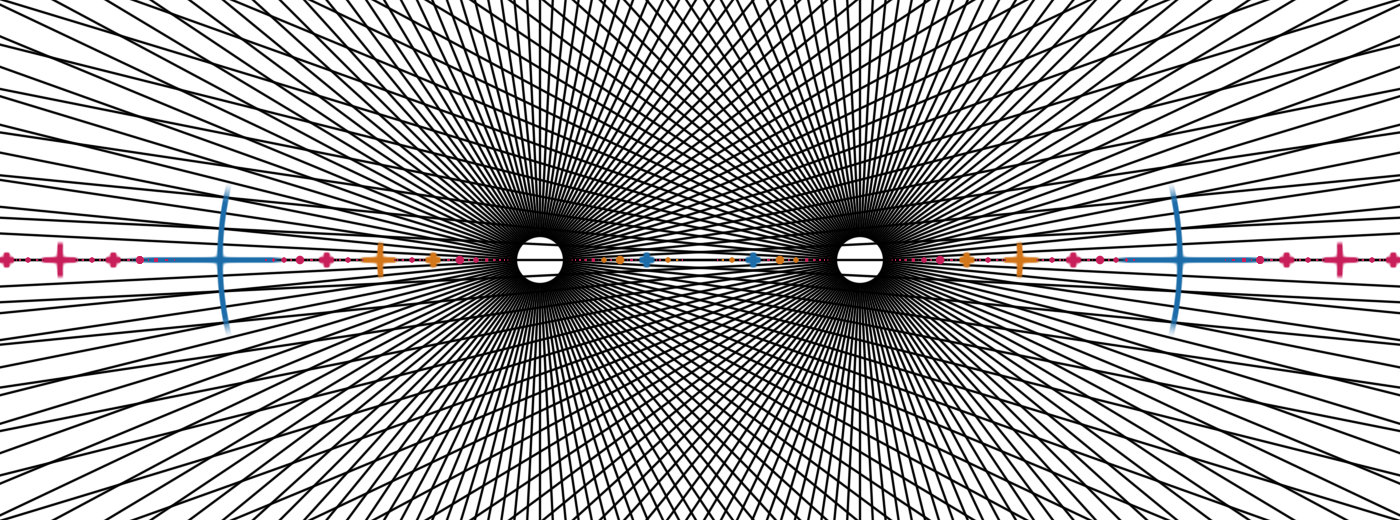
\includegraphics[width=\linewidth]{figures/selection-stations.png}
    \caption{rational stations, per pixel}
    \label{fig:selection-stations}
  \end{subfigure}
  \Description{Left: a staircase plot of the locked rational against the pitch
  ratio, hugging the diagonal, for four order budgets. The budget-two staircase
  has a few wide steps at whole and half-integer ratios; each larger budget
  splits the risers into finer steps that cling closer to the diagonal, and
  around a dashed vertical line marked with the golden ratio the wide steps
  survive every budget. Right: two airy fans of straight lines radiating from
  two ringed holes, and along the horizontal axis through both, small colored
  marks: wide blue arcs far out on either flank, orange crosses closer in,
  and clusters of crimson ticks crowding toward each hole, with a few marks
  between the holes as well.}
  \caption{\figlead{Which beat wins is best approximation.}
  \textbf{(a)}~The winning character $(p,-q)$ of two parallel families, drawn
  as the rational $p/q$ it locks to, against the pitch ratio $\rho$, as the
  order budget grows from $2$ to $16$: a mode-locking staircase whose plateaus
  are the convergents of $\rho$'s continued fraction, each budget splitting
  the risers of the last. Near the golden ratio $\varphi$ (dashed), the
  worst-approximable number, the coarse steps survive every budget: the
  fringe desert. \textbf{(b)}~The same arithmetic as geography.
  Two radial pencils: the local pitch ratio of their index gradients sweeps
  through the rationals along the axis, and each rational the amplitude
  weight admits owns a commensurate pocket, marked by the level sets of the
  per-pixel \emph{winning} character wherever that winner is beyond first
  order and $\mu_k\le1/4$: blue at order two, orange at three and four,
  crimson deeper, the staircase's own hierarchy laid on the ground. The
  first-order sea between the pockets is the moir\'e the render itself
  shows, so it gets no overlay. Computed by the reduction of this section;
  the render never saw the curves.}
  \label{fig:selection}
\end{figure*}

In two dimensions the gradients need not be collinear, and the object that
replaces the continued fraction is a lattice: the candidate beat frequencies
$\{k_1\nabla\idx_1+k_2\nabla\idx_2 : k\in\Z^2\}$ are the integer combinations
of the two carrier gradients, and the slowest character at \emph{any} order is
the shortest nonzero vector of that lattice. In rank two the shortest vector
is not hard: Lagrange--Gauss reduction, the lattice form of the continued
fraction and of Euclid's algorithm, finds it exactly in a handful of
iterations~\cite{NguyenStehle2009Gauss}. \Moire{} therefore runs the
reduction \emph{per pixel}: eight fixed iterations with the integer
coordinates carried along (once a step fails to shrink, later steps rediscover
the same failure, so the unroll needs no termination flag), then the weighted
merit \eqref{eq:merit} minimized over the reduced short vector and a bounded
window around it. The window matters because the weighted winner need not be
a shortest vector: a longer lattice vector can carry smaller integer
coordinates. The six characters with $\lvert k_i\rvert\le2$ remain as a
floor, and the reduction is licensed by the gradients: it runs where both
index gradients are closed-form (\S\ref{sec:catalog}), while a walking
family's gradient is a screen-space difference whose per-quad noise the
reduction would read as slow high-order characters, so those pairs keep the
order-two floor.

The cap it replaces was not a small concession. Over $\selTrials$ random
carrier pairs within a factor of four in pitch, a visible fringe exists
($\min_k\mu_k<1/4$ at order $\le\selTruthOrder$) that the
$\lvert k_i\rvert\le2$ scan declares absent in $\selCapMiss$ cases,
$\selCapMissPct\%$ of the visible fringes, clustering at pitch ratios near
$3$; the shipped bounded scan misses $\selShipMiss$ and names the exhaustive
winner in $\selShipAgreePct\%$ of trials
(\texttt{tools\pslash exp\pslash convergents.mjs}). Figure~\ref{fig:pitch3}
shows what the difference looks like: at a $3{:}1$ pitch ratio the visible
moir\'e is the character $(3,-1)$, which no order-two set contains, so the
criterion read blank while the fringe stood in the render, and the envelope,
whose sweep schedule is chosen by this scan
(\S\ref{sec:envelope}), washed it out. On pairs whose local ratio varies
across the frame, the stations of the convergent ladder become \emph{places}
(Figure~\ref{fig:selection}b).

\begin{figure}[t]
  \centering
  \begin{subfigure}{0.32\linewidth}
    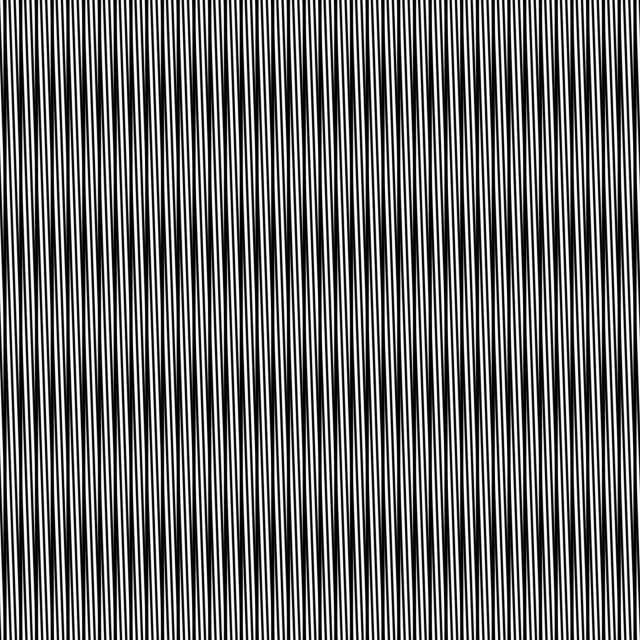
\includegraphics[width=\linewidth]{figures/pitch3-render.png}
    \caption{render}
  \end{subfigure}\hfill
  \begin{subfigure}{0.32\linewidth}
    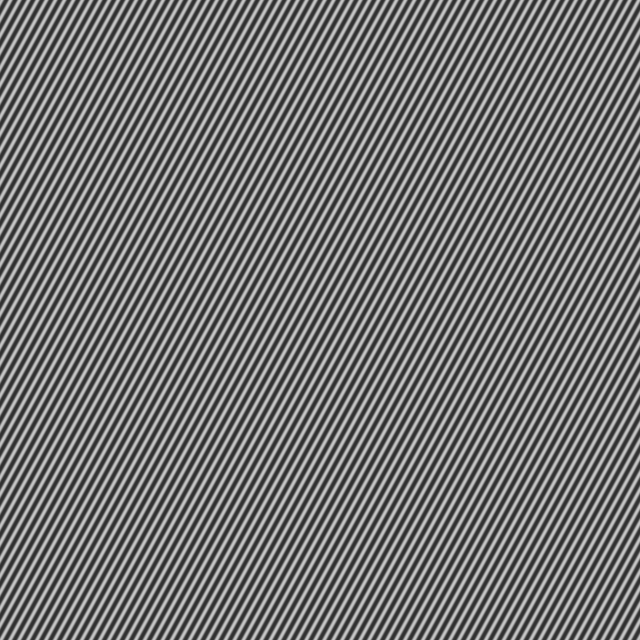
\includegraphics[width=\linewidth]{figures/pitch3-diag.png}
    \caption{diagonal sweep}
  \end{subfigure}\hfill
  \begin{subfigure}{0.32\linewidth}
    
\includegraphics[width=\linewidth]{figures/pitch3-sched.png}
    \caption{$w=(1,3)$}
  \end{subfigure}
  \Description{Three square panels. The first is a dense field of near-vertical
  hairlines whose density waves gently in broad horizontal bands. The second is
  a flat field of fine vertical stripes with no broad bands at all. The third
  is four smooth broad horizontal gray bands with the fine stripes gone.}
  \caption{\figlead{The $3{:}1$ fringe no order cap can hold.} Two line
  families at pitches $15$ and $5$, twisted $2^\circ$. \textbf{(a)}~The render
  carries a broad $(3,-1)$ fringe. \textbf{(b)}~The mean ink over the diagonal
  sweep, which preserves every zero-sum character at once and is all a fixed
  convention can offer: the fringe is not zero-sum, so it washes out, and what
  survives is the fast $(1,-1)$ difference at carrier scale, structure but not
  a fringe. \textbf{(c)}~The mean over the schedule $w=(1,3)$ that the
  per-pixel reduction certifies ($3w_1-1\cdot w_2=0$): the fringe survives the
  average exactly. Both averages are the construction of
  \S\ref{sec:envelope} at $48$ taps and contrast $3$.}
  \label{fig:pitch3}
\end{figure}

\subsection{The envelope view}
\label{sec:envelope}

$\bar\alpha$ is a quantity, so it can be drawn, and drawing it gives the author
the fringe system with the carrier removed. The obvious way to get such a picture
is to blur the render, and it is the wrong way: a blur is a kernel in pixels, so
it changes under zoom, it softens every real edge along with the carrier, and its
width has to be retuned whenever the pitch changes.

Look again at the hypothesis of Theorem~\ref{thm:fringe}. Over the averaging
segment every family's index advances by the \emph{same} amount---that is what
$D$ constant means---so the entire stack is a one-parameter object. Advance every
layer's index together by $u$ and average over $u\in[0,1)$:
\begin{equation}
  \bar\alpha(p) \;=\; \int_0^1 \alpha\big(p;\; \idx_i \mapsto \idx_i + u\big)\,\mathrm{d}u.
  \label{eq:meanink}
\end{equation}
This is an average over \emph{index}, not over space. No sample is taken off
center, so nothing is blurred; the result is the theorem's own $\bar\alpha$ at the
full resolution of the frame, and it is identical at every zoom. Since the
integrand is periodic in $u$ with period exactly $1$, a uniform grid of $M$ nodes
integrates every harmonic exactly except those at nonzero multiples of $M$,
the aliasing algebra of $M$-bucket phase-shifting
interferometry~\cite{Bruning1974Digital, Surrel1996Design}, of which this view
is a synthetic instance, and the integrand's harmonic content decays fast
enough that $M=\envTaps$ leaves an error far below one color step. Every
``averaged ink'' panel in this paper is \eqref{eq:meanink} at $M=\envTaps$, and
it is a toggle in \Moire{}, not a post-process.

Written that way, \eqref{eq:meanink} is an integral over the diagonal of the
\emph{index torus} $[0,1)^K$, one circle per family, and the choice of the
diagonal is exactly Theorem~\ref{thm:fringe}'s hypothesis rather than a
convenience. The alternative deserves stating, because we implemented it
first. Sweeping a rigid translation of the whole stack is a motion the layers
could really make, where advancing an index is bookkeeping; it is also unusable:
the taps then sample a two-dimensional disc for strokes that cover a few percent
of it, so a handful of taps carry the answer and the rest carry noise. Sixty-four
of them left the carrier standing and the fringes mottled. The diagonal is a
fiction---no motion of the layers realizes it---and that is precisely why
its average is the theorem's.

Which direction to sweep is the character choice of \S\ref{sec:visibility} over
again, and one rule settles it: averaging along a direction
$w=(w_1,\dots,w_K)$ of the torus annihilates every character
$k$ with $k\cdot w\neq0$ and preserves those with $k\cdot w=0$, so \emph{the
sweep must run orthogonal to the character it is meant to keep}. The diagonal
$w=(1,1)$ preserves $\idx_1-\idx_2$ and averages the sum moir\'e away;
$w=(1,-1)$, the second family swept backwards, preserves the sum; and a
second-order beat such as $2\idx_1-\idx_2$ needs $w=(1,2)$, without which the
view erases a fringe that is bold in the render. \Moire{} picks $w$ per pixel
from the same character scan the criterion runs, so the view keeps whichever
beat the criterion certifies (\S\ref{sec:selection}); each direction still
covers a whole period of every family, so nothing else about the average
changes.

The rule scales to $K$ layers without amendment, and to any order: the winner
$(k_1,k_2)$ in general rides $w=(\lvert k_2\rvert,\mp k_1)$, so the $(3,-1)$
beat of a $3{:}1$ pitch ratio, which \S\ref{sec:selection} finds by reduction,
is held by $w=(1,3)$ (Figure~\ref{fig:pitch3}). The rule also says something
worth pausing on: the diagonal $w=(1,\dots,1)$ preserves exactly the
\emph{zero-sum} sublattice $\{k:\sum_i k_i=0\}$, every pairwise difference
and every zero-sum ternary character at once. A beat between beats such as
$k=(1,1,-2)$, slow wherever $\nabla\idx_1+\nabla\idx_2\approx2\nabla\idx_3$,
rides the diagonal for free; three ring families arrange that conspiracy
over half the frame when $2/s_3=1/s_1+1/s_2$, the harmonic mean, and the
fringes that appear there belong to no pair (the second harmonic of the
third family carries them, so its duty cycle must stay off one half). What
costs a deviation is only a winning character that is \emph{not} zero-sum,
and the deviation must be chosen against every layer it touches: deviating
the top pair's rates for a sum beat can scramble a slower difference beat
the second layer makes with the \emph{third}, a fringe that stands in the
render and washes from the view, which is how our two-layer scan first
failed on three. \Moire{} therefore scans all pairs among the three topmost
families, plus the zero-sum ternaries, and spends a rate deviation only on
the global winner (supplemental \S S3;
\texttt{tools/exp/ternary.mjs} reproduces the harmonic-mean prediction).

\paragraph{One solve, many taps.}
The cost, done naively, is $M$ full evaluations of every layer, and for a
walking family one evaluation is the search of \S\ref{sec:inverse}, so $\envTaps$
of them per pixel is a stall rather than a view: implemented that way, the
envelope ran at five frames a second on the tool's own opening preset.

It need not, because advancing an index by less than one does not change
\emph{which} members are nearby. The solver is asked once per pixel for a
\emph{phase sample}
\begin{equation}
  \Pi(p) \;=\; \big(\,z,\; z^{\uparrow},\; z^{\downarrow},\; \ell\,\big),
  \label{eq:phasesample}
\end{equation}
the signed distances to the nearest member and to the two flanking it, plus a
floor $\ell$ for everything that does not slide (a saturated solve's guard,
the hole at a pencil's center, the hyperbola's missing innermost neighbor;
separating these from the residual is what keeps the average from inventing
ink where there is nothing to slide onto). A tap at $u$ then reads
\begin{equation}
  d(p;u) \;=\; \max\Big(\min_{k\in\{z,z^{\uparrow},z^{\downarrow}\}} \lvert k - u\,\mathrm{gap} \rvert,\; \ell\Big),
  \label{eq:slide}
\end{equation}
with $\mathrm{gap}=\lvert z^{\uparrow}-z\rvert$ the \emph{local} member gap,
so a tap covers one period of \emph{this} family at \emph{this} point
whatever the pitch does across the frame, which is what the pencil needs,
its gap growing with radius. For the nine phase families \eqref{eq:slide}
reproduces the re-solved distance exactly, in nine instructions. For the
pencil and the walking families it is first-order per tap yet exact for the
integral's purpose, because the measured local gap is precisely one carrier
period; the alternative, advancing the \emph{phase} at the nominal rate, has
no unit period on a walking family at all (radii grow while every pose stays
put) and leaves visible residue in the view. Two implementation facts belong
in the open. The solver runs these views with the guard widened to a full
pitch, since Eq.~\ref{eq:guard}'s $\tfrac34 s$ would prove away the flanking
members the sample needs. And the search still runs once per pixel while the
sweep is arithmetic: median envelope frame times went from hundreds of
milliseconds to within the 60\,Hz budget.

Each family realizes the advancing index in its own parameter: a phase shift
for the level-set families, a rotation for the radial pencil, a translation for
a lattice. A lattice's index is a \emph{pair}, so which combination of its two
generators rides the sweep, and which way, is the character choice of
\S\ref{sec:visibility} once more, and it must be made per point, or fringes
plainly present in the render vanish from the view. Those details, and the
contrast pivot the view expands about, are in the supplemental material (\S S3).

One caveat remains, and it is structural rather than a matter of implementation.
The average is over the diagonal, so where Theorem~\ref{thm:fringe}'s hypothesis
fails, where $\het$ is large, the view still shows $\Phi(D)$ faithfully, but
$\Phi(D)$ is no longer what the eye will average. The two are therefore meant to be
read together: the envelope jointly with the ratio map beside it.

\subsection{Verification}

Theorem~\ref{thm:fringe} is a claim about a rendered image, so we measured it.
For \fringeScenes{} scene pairs spanning straight, curved, isotropic,
anisotropic, periodic and aperiodic families (one of them a walking family,
whose index field is the searched-for local one above) we compute the exact
one-period directional mean of the union from the fields themselves, with no
raster and hence no sampler error, and
compare it against $\Phi$ evaluated at the window center. There is no fitting and no free
parameter. Points are excluded on three stated grounds, each the empirical form
of one of the theorem's hypotheses, so what is verified is the conditional
claim: strokes merged ($w_i+b_i>0.45$, the tent's width condition), carrier
bending more than $0.15$\,rad across its own period (the foliation hypothesis),
and gradient varying more than $15\%$ across a period (the constant-gradient
hypothesis). The regime filter uses the $(1,-1)$ ratio alone, which is
conservative: points where only another character of \S\ref{sec:visibility} is
slow are excluded rather than tested, and extending the verification to the
other characters is left open.

% GENERATED by paper/tools/numbers.mjs
\begin{table*}[t]
\caption{\figlead{The fringe law, measured.} Mean and $99$th-percentile absolute
error between the one-period directional mean of the rendered ink and $\Phi(D)$ of
Eq.~\ref{eq:phi}, over samples in the fringe regime $\het\le1/4$. \emph{Swing} is
the range of measured coverage, so it says how much fringe there was to get wrong.
\emph{Light\,/\,dark} are the mean distances of the measured lightest and darkest
deciles from the nearest integer index difference; the ideals are $0$ (light
fringes at $D\in\Z$) and $0.5$ (dark fringes at $D\in\Z+\tfrac12$). Where the
profile plateaus (low swing), the darkest decile spreads across the flat top and
its mean falls short of $0.5$ by construction. \emph{In regime} is the share of admissible samples with $\het\le1/4$. The
last row has none: with those settings no fringe exists, and the criterion says so
without rendering.}
\label{tab:fringe}
% The Families column carries long prose; \small leaves the widest row 11pt
% over the full text width, which prints into the margin.
\footnotesize
\centering
\begin{tabular}{@{}llrrrrcr@{}}
\toprule
Scene & Families & $n$ & mean & p99 & swing & light\,/\,dark & in regime \\
\midrule
\texttt{parallel-rotate} & two line families 6 degrees apart & 14,641 & 0.0000 & 0.0000 & 0.320 & 0.024 / 0.474 & 100\% \\
\texttt{parallel-pitch} & same direction, pitch mismatched by 4 percent & 14,641 & 0.0059 & 0.0189 & 0.326 & 0.026 / 0.470 & 100\% \\
\texttt{circle-circle} & circle families with displaced centres & 6,118 & 0.0000 & 0.0001 & 0.277 & 0.028 / 0.465 & 45\% \\
\texttt{circle-parallel} & circles under lines; D is not periodic in p & 3,952 & 0.0000 & 0.0000 & 0.242 & 0.034 / 0.475 & 27\% \\
\texttt{hexagon-hexagon} & anisotropic metric, hexagons 4 degrees apart & 13,382 & 0.0000 & 0.0000 & 0.260 & 0.024 / 0.475 & 95\% \\
\texttt{square-circle} & two different norms at the same spacing & 3,524 & 0.0000 & 0.0001 & 0.242 & 0.002 / 0.460 & 25\% \\
\texttt{spiral-circle} & aperiodic family: Archimedean spiral over circles & 14,041 & 0.0000 & 0.0001 & 0.243 & 0.031 / 0.461 & 100\% \\
\texttt{parabola-parabola} & curved families, bend mismatched by 8 percent & 484 & 0.0166 & 0.0329 & 0.169 & 0.160 / 0.218 & 100\% \\
\texttt{wave-parallel} & a wave family over lines & 14,641 & 0.0003 & 0.0011 & 0.118 & 0.011 / 0.170 & 100\% \\
\texttt{hyperbola-hyperbola} & rectangular hyperbolae, spacing mismatched by 4 percent & 11,036 & 0.0079 & 0.0214 & 0.640 & 0.123 / 0.430 & 100\% \\
\texttt{walking-circle} & a walking family (member $n$ displaced by $n\delta$) over concentric circles & 11,231 & 0.0159 & 0.0731 & 0.388 & 0.037 / 0.403 & 82\% \\
hyperbola\hspace{0.5pt}-\hspace{0.5pt}parallel & hyperbolae under lines: almost no fringe regime exists & --- & --- & --- & --- & --- & $0$ \\
\bottomrule
\end{tabular}
\end{table*}


Table~\ref{tab:fringe} reports the result. Across $\fringeSamples$ admissible
in-regime samples the mean absolute coverage error is $\fringeMeanErr$ and the
worst $99$th percentile over any scene is $\fringeWorstP$, against a fringe swing of
$0.12$--$0.64$ in coverage. Measured as index-gap from the nearest integer, the
lightest deciles sit at a mean of $\fringeLight$ and the darkest at $\fringeDark$,
against ideals of $0$ and $0.5$. The darkest-decile figure is diluted by the
scenes whose profile plateaus: on a flat top every phase is equally dark, so the
decile spreads across it and its mean distance falls below $0.5$ without any
fringe being out of place.

The last row is the informative one. \texttt{hyperbola-parallel} has \emph{no}
in-regime samples anywhere in the frame: $\het_k>1/4$ for every scanned
character, because a hyperbola family's index gradient sweeps through all
directions while a line family's does not. No low-order fringe forms in that
superposition, only a lattice of crossings, and the criterion says so before
rendering.
